%  TESINA / PROYECTO DE INNOVACIÓN Y/O MEJORA - Formato SENATI

% ------------------------------------------

\documentclass[12pt,a4paper]{report}

% ---------- Idioma y codificación ----------
\usepackage[utf8]{inputenc}
\usepackage[T1]{fontenc}
\usepackage[spanish,es-tabla]{babel}
\usepackage{float}
\decimalpoint

% ---------- Tipografía estilo Times ----------
\usepackage{mathptmx}

% ---------- Márgenes tipo APA (2.5 cm / 1 pulgada) ----------
\usepackage[a4paper,margin=2.5cm]{geometry}

% ---------- Interlineado ----------
\usepackage{setspace}
\onehalfspacing
%doble espacio estricto (APA puro)esta:
% \doublespacing

% ---------- Encabezado y pie de página ----------
\usepackage{fancyhdr}
\pagestyle{fancy}
\setlength{\headheight}{14.5pt}
\fancyhf{}
\fancyhead[L]{Sistema web de gestión tributaria predial con Machine Learning} 
\fancyhead[R]{\thepage}
\renewcommand{\headrulewidth}{0.4pt}
% Las primeras páginas de capítulo usan el estilo 'plain': que conserven encabezado y número
\fancypagestyle{plain}{%
  \fancyhf{}
  \fancyhead[L]{Sistema web de gestión tributaria predial con Machine Learning}
  \fancyhead[R]{\thepage}
  \renewcommand{\headrulewidth}{0.4pt}
}

% ---------- Otros paquetes útiles ----------
\usepackage{graphicx}
\usepackage{tikz}
\usetikzlibrary{positioning,shapes.geometric,arrows.meta}
\usepackage{caption}
\usepackage{booktabs}
\usepackage{longtable}
\usepackage{enumitem}
\usepackage{amsmath,amssymb}
\usepackage[hidelinks]{hyperref}
\usepackage{csquotes}
\usepackage[
  backend=biber,
  style=apa,
  sorting=nyt
]{biblatex}
\DeclareLanguageMapping{spanish}{spanish-apa} % APA en español ("y", "s.f.", etc.)
\addbibresource{referencias.bib}
% Permite cortar los DOI/URL largos sin abrir espacios entre caracteres
\setcounter{biburlnumpenalty}{100}
\setcounter{biburlucpenalty}{100}
\setcounter{biburllcpenalty}{100}
\biburlbigskip=0mu plus 0.5mu
\biburlnumskip=0mu plus 0.5mu
\biburlucskip=0mu plus 0.5mu
\biburllcskip=0mu plus 0.5mu

\graphicspath{{imagenes/}}

% Inserta la imagen si existe; si no, muestra un recuadro marcador (no rompe la compilación)
\newcommand{\imgopt}[2]{%
  \IfFileExists{imagenes/#2}{\includegraphics[width=#1\textwidth]{#2}}%
  {\fbox{\parbox[c][4cm][c]{0.6\textwidth}{\centering\textit{[Insertar imagen: \detokenize{#2}]}}}}%
}

% ---------- Numeración de capítulos tipo "1.1.1." ----------
\setcounter{secnumdepth}{4}
\setcounter{tocdepth}{4}

% ---------- Numeración de Tablas/Figuras "Tabla 1", "Figura 1" (sin capítulo) ----------
\usepackage{chngcntr}
\counterwithout{table}{chapter}   % que no se reinicien en cada capítulo
\counterwithout{figure}{chapter}
\renewcommand{\thetable}{\arabic{table}}
\renewcommand{\thefigure}{\arabic{figure}}

\title{Sistema web de gestión tributaria predial con Machine Learning}
\author{[Tus nombres]}
\date{[Mes y año]}

\begin{document}


% ---------- CARÁTULA---------- 

\begin{titlepage}
\centering

\includegraphics[width=0.5\textwidth]{logo_senati.png}\par
\vspace{0.5cm}

{\large SERVICIO NACIONAL DE ADIESTRAMIENTO EN TRABAJO INDUSTRIAL\par}
\vspace{0.2cm}
{\large\bfseries DIRECCIÓN ZONAL: LIMA -- CALLAO\par}
\vspace{0.2cm}
{\large ESCUELA DE TECNOLOGÍA DE LA INFORMACIÓN\par}
\vspace{0.2cm}
{\large CFP LUIS CÁCERES GRAZIANI\par}
\vspace{0.2cm}
{\large\bfseries INGENIERÍA DE SOFTWARE CON INTELIGENCIA ARTIFICIAL\par}
\vspace{0.2cm}
{\large Proyecto de Innovación y/o Mejora\par}
\vspace{0.2cm}
{\large Nivel Profesional Técnico/ Técnico Operativo\par}
\vspace{1.5cm}
% sad
{\Large\bfseries ``IMPLEMENTACIÓN DE UN SISTEMA WEB DE GESTIÓN TRIBUTARIA PREDIAL PARA OPTIMIZAR LA COBRANZA Y ESTIMAR EL RIESGO DE MOROSIDAD USANDO MACHINE LEARNING''\par}
\vspace{1.5cm}

{\bfseries Autores:\par}
\vspace{0.2cm}
{\large Renzo Alexis Pérez Gonzales\par}
{\large Xavier Eulices Gerdez Villalobos\par}
\vspace{1cm}

{\bfseries Asesor:\par}
\vspace{0.2cm}
{\large Mg. José Armando Tiznado Ubillus\par}
\vfill

{\bfseries Lima -- Callao\par}
\vspace{0.2cm}
{\bfseries 2026\par}
\end{titlepage}

\pagenumbering{arabic}


% ----------AGRADECIMIENTO----------

\chapter*{Agradecimiento}
\addcontentsline{toc}{chapter}{Agradecimiento}

En esta ocasión, mediante el presente trabajo quiero dedicar unas palabras a todas esas personas que me apoyaron y nunca me dejaron solo durante este proceso, ya que sin ellos nada de esto habría sido posible.
En primer lugar, agradezco a mis padres por su guía y motivación constante. Mis profesores, que me compartieron todo su conocimiento y me enseñaron la pasión por la tecnología. Mi hermanita, que siempre creyó en mí y nunca dudo de mis habilidades. Mis amigos, que me mantenían siempre feliz y sonriente.



% ----------DEDICATORIA----------
\chapter*{Dedicatoria}
\addcontentsline{toc}{chapter}{Dedicatoria}

A mi familia, que fue el pilar de mi formación y me apoyaron incondicionalmente desde el día 1, gracias por todo el sacrificio y por todo el cariño que me han dado siempre.

A mis profesores, por guiarme y hacer posible el crecimiento tanto personal como profesional que he conseguido.
A mí mismo, por no rendirme en el camino, por mantener la misma ilusión y las mismas ganas de aprender y de crecer.


% ----------RESUMEN----------
\chapter*{Resumen}
\addcontentsline{toc}{chapter}{Resumen}

El presente proyecto tiene como finalidad el desarrollo de un sistema informático web para la Municipalidad de San Bartolo, orientado a reemplazar el software de gestión municipal actualmente en uso, el cual fue desarrollado en Visual FoxPro 9 como una aplicación de escritorio local dependiente de un servidor físico. Esta dependencia limita la flexibilidad operativa de la institución, restringiendo el acceso al sistema únicamente a los equipos conectados a dicha infraestructura y dificultando su mantenimiento y escalabilidad a largo plazo.

Ante esta problemática, se propone la migración del sistema hacia una arquitectura web, que permita a los funcionarios municipales acceder a la plataforma desde cualquier ubicación con conexión a internet, eliminando la dependencia de un servidor local. El nuevo sistema conservará y optimizará las funcionalidades principales del software existente, entre las cuales se encuentran el registro de personas y propietarios, la gestión de propiedades, el procesamiento de transferencias de propiedad por concepto de venta, la baja de propiedades y el registro de propiedades heredadas, procesos característicos de la gestión catastral municipal.

La metodología de desarrollo contempla, en una primera etapa, el acceso y exploración del sistema actual con el objetivo de identificar de manera detallada sus funcionalidades, con el propósito de replicarlas e incorporar mejoras tanto a nivel tecnológico como de experiencia de usuario. El desarrollo se inicia con la implementación del módulo de autenticación (login), componente fundamental al tratarse de un sistema web que requiere control de acceso mediante usuario y contraseña, gestionado mediante tokens JWT y contraseñas cifradas con bcrypt.

Para la construcción del sistema se ha definido un stack tecnológico compuesto por Node.js con el framework NestJS y TypeScript para el desarrollo del backend, React junto con Tailwind CSS y Vite para la interfaz de usuario, y PostgreSQL con Prisma ORM como sistema gestor de base de datos relacional. Esta selección responde a criterios de escalabilidad, mantenibilidad del código y compatibilidad con el equipo de desarrollo.

Asimismo, el proyecto incorpora un modelo de Machine Learning que estima el riesgo de morosidad de los contribuyentes a partir del historial de pagos y deudas, con el fin de priorizar la cobranza y dotar al sistema de capacidades de análisis predictivo sobre los datos administrados.


% ----------ÍNDICES----------

\tableofcontents
\listoftables
\listoffigures
% Anexos no tiene comando automático: se arma a mano al final si hace falta.

% ----------INTRODUCCIÓN----------
\chapter*{Introducción}
\addcontentsline{toc}{chapter}{Introducción}

La gestión municipal de propiedades, registro de propietarios, transferencias, herencias y bajas; requiere información actualizada y de fácil acceso para un servicio eficiente al ciudadano. En la Municipalidad de San Bartolo, este proceso se sostiene sobre un software desarrollado en Visual FoxPro 9, instalado como aplicación de escritorio y dependiente de un servidor físico local. Esta dependencia se ha vuelto especialmente crítica ante el actual proceso de reubicación del local municipal, situación que expone los riesgos de un sistema atado a infraestructura física: interrupciones del servicio, pérdida temporal de acceso a la información y complicaciones logísticas que un sistema web evitaría al permitir el acceso desde cualquier punto con conexión a internet.

Esta debilidad no es aislada. En el Perú, la mayoría de los más de 1,800 gobiernos locales no cuenta con un catastro urbano adecuadamente implementado, y solo unos pocos distritos han consolidado sistemas modernos de gestión territorial, evidenciando un desarrollo tecnológico municipal desigual. El mismo patrón se repite a escala internacional: informes de la OCDE-BID y de las Naciones Unidas coinciden en que, si bien los gobiernos nacionales avanzan en digitalización, ese progreso no siempre llega con la misma fuerza al nivel local, donde se gestionan los servicios más cercanos al ciudadano.

Frente a este contexto, el proyecto propone desarrollar un sistema web para la Municipalidad de San Bartolo que elimine la dependencia de un servidor físico, permitiendo el acceso remoto y continuo de los funcionarios incluso ante eventualidades como una mudanza institucional. La propuesta contempla el análisis de las funcionalidades del sistema actual para replicarlas y mejorarlas bajo una arquitectura más moderna y escalable.

Como valor agregado, el proyecto contempla incorporar inteligencia artificial dentro del software, lo cual permitiría atender la problemática desde distintos niveles. A nivel local, un modelo de Machine Learning que estime el riesgo de morosidad de los contribuyentes ayudaría a priorizar la cobranza con recursos limitados, una restricción común en municipios de escala similar. A nivel nacional, su adopción progresiva contribuiría a reducir la brecha entre los pocos municipios con sistemas modernos y la mayoría que aún opera de forma manual. A nivel internacional, la iniciativa se alinea con el impulso de organismos como la OCDE y la UNESCO hacia un uso responsable de la IA en la administración pública, además de experiencias ya en marcha en gobiernos locales de la región que regulan su uso. Así, el proyecto no solo resuelve una necesidad puntual de San Bartolo, sino que se inserta en una tendencia más amplia de modernización de la gestión pública local.


% CAPÍTULO I: GENERALIDADES DE LA EMPRESA
\chapter{Generalidades de la Empresa}

\section{Datos Generales de la Empresa}

\subsection{Reseña Histórica de la Empresa}
Consultoría Informática es un negocio unipersonal a cargo del señor Iván Casariego, dedicado al desarrollo y venta de software para municipalidades, con domicilio en San Juan de Miraflores, Lima. La empresa inició sus operaciones en 1998, cuando su fundador identificó la necesidad de las entidades públicas locales de contar con herramientas tecnológicas propias para automatizar y ordenar su gestión administrativa, en un contexto donde muchas municipalidades aún dependían de procesos manuales.

Desde entonces, y a lo largo de más de dos décadas de trabajo, Consultoría Informática ha ampliado progresivamente su alcance, llegando a prestar servicios a diversas municipalidades del país mediante el desarrollo de sistemas de software adaptados a sus necesidades. Este crecimiento le ha permitido consolidarse como un proveedor con experiencia dentro de este segmento tecnológico especializado.

Es importante señalar que Iván Casariego no limita su actividad empresarial únicamente al rubro de software: a lo largo de los años ha diversificado sus negocios, incursionando también en el alquiler de equipos, la venta de vehículos y actividades vinculadas a la pesca. Cada uno de estos negocios funciona de manera independiente entre sí, lo que refleja una trayectoria empresarial diversificada, aunque Consultoría Informática se mantiene como su unidad de negocio enfocada específicamente en soluciones tecnológicas para el sector municipal, siendo este el ámbito en el que se desarrollan las prácticas pre-profesionales.
\subsection{Quiénes Somos}
Consultoría Informática es un negocio unipersonal liderado por el señor Iván Casariego, especializado en el desarrollo y la venta de software orientado a la gestión municipal. Con presencia en San Juan de Miraflores y más de 25 años de trayectoria en el rubro tecnológico, nos dedicamos a diseñar soluciones informáticas que permiten a las municipalidades optimizar y modernizar sus procesos administrativos. Nuestro compromiso es acompañar a las entidades públicas locales con herramientas confiables y adaptadas a sus necesidades, contribuyendo así a una gestión municipal más eficiente y ordenada.

\subsection{Razón Social}

\begin{table}[h]
\centering
\caption{Datos de la empresa}
\label{tab:empresa}
\begin{tabular}{ll}
\toprule
\textbf{Nombre comercial} & Consultoría Informática \\
\textbf{Razón social} & Adolfo Iván Casariego Aguilar (persona natural con negocio) \\
\textbf{RUC} & 10107080321 \\
\textbf{Rubro} & Desarrollo y venta de software para municipalidades \\
\textbf{Distrito} & San Juan de Miraflores \\
\textbf{Dirección} & Jr. Jorge Basadre 297, Lima 15801, Perú \\
\bottomrule
\end{tabular}
\end{table}

\subsection{Logo de la Empresa}

\begin{figure}[H]
  \centering
  \caption{Logo de la Empresa}
  \label{fig:logo_empresa}
  \imgopt{0.7}{logo_empresa.png}
  \par\footnotesize \textit{Nota.} Logo de Consultoría Informática, proporcionado por la empresa.
\end{figure}

\subsection{Localización de la Empresa}
La Figura~\ref{fig:localizacion} muestra la ubicación de la empresa, en Jr. Jorge Basadre 297, San Juan de Miraflores, Lima 15801.

\begin{figure}[H]
  \centering
  \caption{Localización de la Empresa}
  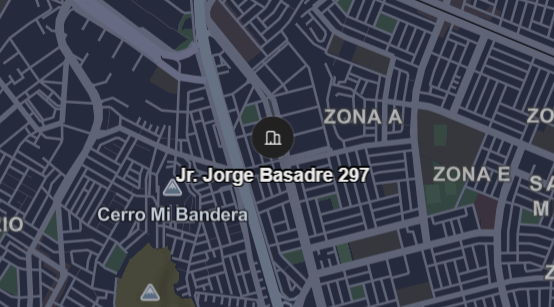
\includegraphics[width=0.55\textwidth]{ubicacion.png}
  
  \label{fig:localizacion}
  \par\footnotesize \textit{Nota.} Elaboración propia a partir de Google Maps (2026).
\end{figure}

\section{Misión, Visión, Objetivo y Valores de la Empresa}

\subsection{Misión}
Diseñar, desarrollar e implementar soluciones informáticas confiables, seguras y adaptadas a las necesidades específicas de las municipalidades peruanas, contribuyendo a la modernización de su gestión administrativa y a la mejora continua de la atención al ciudadano, mediante un servicio técnico cercano y comprometido con cada entidad cliente.

\subsection{Visión}
Consolidarnos, para el año 2030, como la empresa referente a nivel nacional en la estandarización y modernización de los sistemas de gestión municipal, reconocida por la calidad, escalabilidad y sostenibilidad de sus soluciones tecnológicas, y por su aporte a la reducción de la brecha digital entre los gobiernos locales del Perú.

\subsection{Objetivo}
Normalizar progresivamente los sistemas informáticos utilizados por las municipalidades del Perú, reemplazando los desarrollos particularizados y dependientes de infraestructura física o de una sola persona por soluciones web estandarizadas, escalables y de fácil mantenimiento, que optimicen los procesos de gestión municipal y faciliten el acceso a la información para la toma de decisiones.

\subsection{Valores de la Empresa}

\begin{itemize}
  \item \textbf{Compromiso:} con la calidad del servicio brindado a cada municipalidad cliente y con el cumplimiento de los plazos y requerimientos acordados.
  \item \textbf{Confiabilidad:} garantizando la seguridad, disponibilidad e integridad de la información gestionada por los sistemas desarrollados.
  \item \textbf{Innovación:} incorporando de manera constante nuevas tecnologías (como la inteligencia artificial) que aporten valor a la gestión pública local.
  \item \textbf{Responsabilidad social:} entendiendo que las soluciones desarrolladas impactan directamente en la calidad del servicio que las municipalidades ofrecen a los ciudadanos.
  \item \textbf{Adaptabilidad:} ajustando las soluciones tecnológicas a la realidad, presupuesto y capacidad operativa de cada municipalidad atendida.
\end{itemize}

\section{Producto, Mercado y Cliente}

\subsection{Producto}

Consultoría Informática ofrece un sistema integral de gestión municipal orientado al área de rentas y trámites documentarios, que permite automatizar procesos como el registro de contribuyentes y propietarios, la administración del catastro urbano, el procesamiento de transferencias y bajas de propiedades, y la generación de reportes para la toma de decisiones. El producto se entrega actualmente como software de escritorio, aunque se encuentra en proceso de migración hacia una arquitectura web que permita un acceso más flexible y una mejor experiencia de uso para el personal municipal.

\subsection{Mercado}

El mercado objetivo de la empresa está conformado por el sector público local a nivel nacional, específicamente por las municipalidades distritales y provinciales del Perú que requieren digitalizar o modernizar su gestión administrativa. Dado que, según cifras del RENAMU, una parte significativa de los gobiernos locales del país aún no cuenta con sistemas digitales adecuados para sus procesos, este segmento representa un mercado con demanda potencial de crecimiento sostenido, especialmente en municipios distritales de mediana y pequeña escala.

\subsection{Cliente}

Los clientes de Consultoría Informática son las municipalidades peruanas, principalmente aquellas de escala distrital, que requieren soluciones tecnológicas adaptadas a sus procesos internos de gestión de rentas, catastro y trámites documentarios. Entre estos clientes se encuentra actualmente la Municipalidad de San Bartolo, entidad para la cual se desarrolla el presente proyecto de innovación.

\section{Organigrama de la Empresa}

\begin{figure}[H]
  \centering
  \caption{Organigrama de la Empresa}
  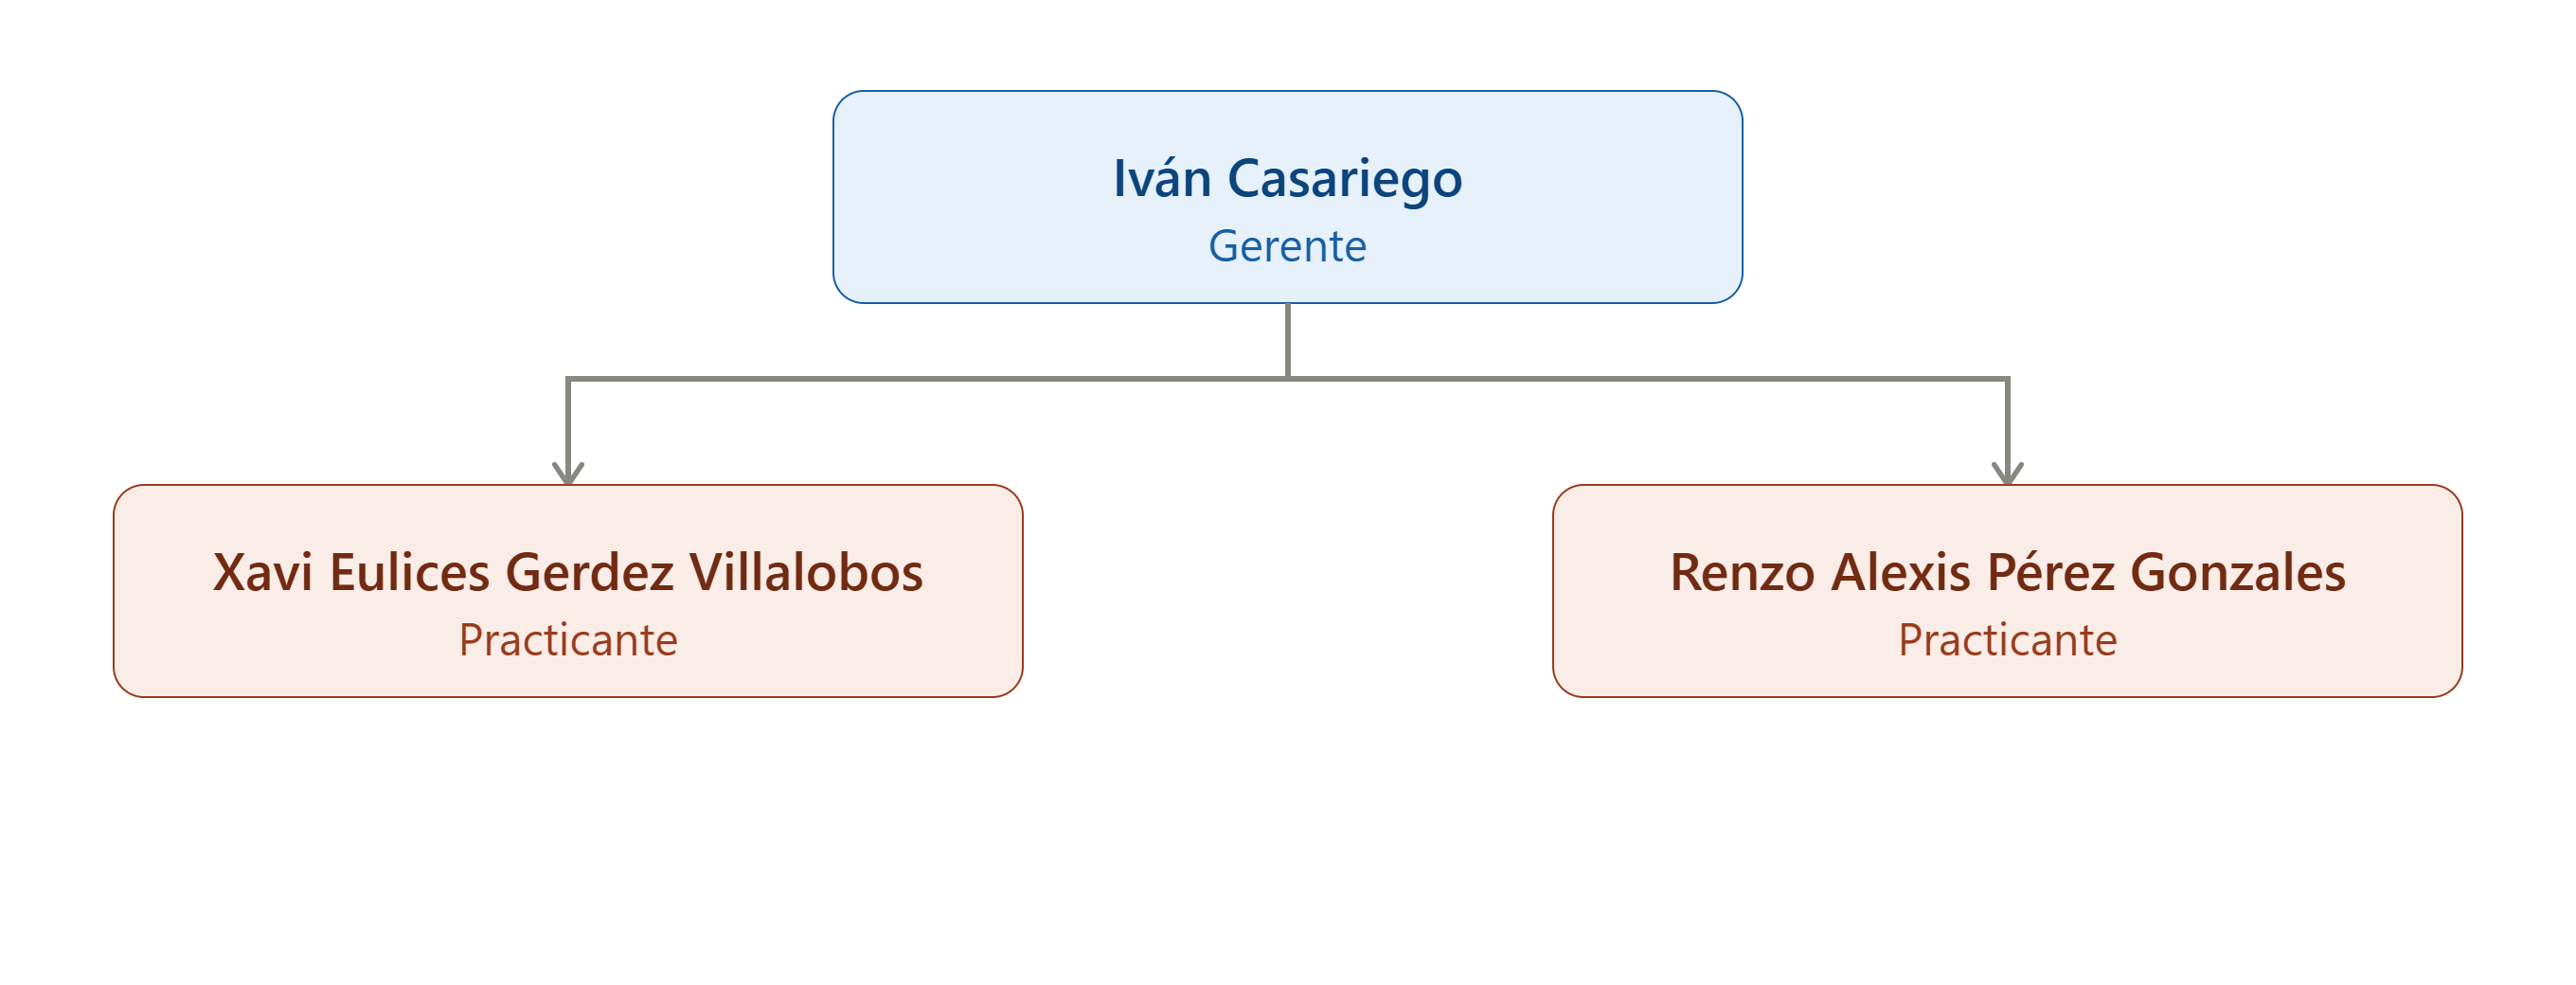
\includegraphics[width=0.9\textwidth]{organigrama.png}
  \label{fig:organigrama}
  \par\footnotesize \textit{Nota.} Elaboración propia. Estructura organizacional de Consultoría Informática y sus niveles jerárquicos.
\end{figure}

\section{Otra información relevante de la Empresa donde se desarrollará el Proyecto}

\subsection{Contexto del Proyecto: Municipalidad de San Bartolo}
El presente proyecto se desarrolla para la Municipalidad de San Bartolo, cliente de Consultoría Informática, que utiliza Sispredios para administrar el registro de contribuyentes y predios, la emisión de deudas del impuesto predial y los arbitrios, la caja y la cobranza ordinaria y coactiva. El sistema funciona instalado en los equipos de la municipalidad y depende de un servidor físico local, situación que se ha vuelto crítica con el proceso de reubicación del local municipal, ya que cualquier traslado del servidor interrumpe el acceso a la información.

En este contexto, la empresa decidió migrar Sispredios a una plataforma web estandarizada que pueda reutilizarse con otras municipalidades. La primera versión de la nueva base de datos agrupa la información en ocho dominios (administración, contribuyentes, catastro y predios, vehicular, parámetros tributarios, deuda y caja, cobranza y coactivo, y licencias) y, sobre el historial de deudas y pagos registrado durante años, se incorpora un modelo de Machine Learning para estimar el riesgo de morosidad.

% CAPÍTULO II: PLAN DE PROYECTO DE INNOVACIÓN / MEJORA / CREATIVIDAD

\chapter{Plan de Proyecto de Innovación / Mejora / Creatividad}

\section{Identificación del Problema Técnico en la Empresa}

\subsection{Problema Local de la Empresa}

Consultoría Informática desarrolla y vende software de gestión a municipalidades, y uno de sus productos es Sispredios, un sistema de gestión tributaria predial desarrollado en Visual FoxPro 9 como aplicación de escritorio. Se trata de un sistema de gran tamaño: el análisis de sus archivos muestra 219 formularios, 202 reportes y 252 tablas en su base de datos principal, que ocupa cerca de 3,5 GB, con alrededor de 1,9 millones de registros en su tabla de cuenta corriente y más de un millón de registros de pagos. % VERIFICAR el significado de la tabla de cuenta corriente al leer el código

Esta tecnología, además, ya no cuenta con respaldo del fabricante: Microsoft mantuvo el soporte extendido de Visual FoxPro hasta enero de 2015 \parencite{taft2007}. A esto se suma que el sistema funciona instalado en equipos locales, por lo que su uso queda limitado a la infraestructura física de cada entidad, y que cada municipalidad atendida cuenta con una solución distinta, construida de manera particular.

Al aplicar el método de Pareto se identificó el problema principal: \textit{falta de estandarización y sostenibilidad en el desarrollo y soporte de los sistemas de software entregados a las municipalidades.} Este problema se origina en cuatro causas. La primera es la \textit{falta de estandarización en los sistemas desarrollados}, ya que cada municipalidad cuenta con una solución distinta, lo que dificulta el mantenimiento, la escalabilidad y la reutilización de código entre proyectos. La segunda son las \textit{interfaces de usuario poco intuitivas, con un diseño UI/UX obsoleto e incómodo}, propio de aplicaciones de escritorio antiguas, que dificulta el uso cotidiano del personal municipal. La tercera son las \textit{demoras en la atención de soporte técnico}, debido a que el conocimiento y la carga de trabajo se concentran en una sola persona y no existen procesos ni personal dedicado exclusivamente a las incidencias, situación que se agrava al depender de una tecnología sin soporte oficial.

La cuarta causa es la \textit{limitación en el acceso a información estadística}: los sistemas actuales no facilitan la generación ni la consulta de reportes consolidados, y el historial de pagos y deudas acumulado durante años no se aprovecha para anticipar la morosidad ni para priorizar la cobranza, por lo que la gestión de cobro se vuelve reactiva. % VERIFICAR con el encargado de la empresa

Esta situación se refleja en la propia instalación de Sispredios. Algunos de sus programas auxiliares conservan rutas fijas a carpetas de otras municipalidades atendidas por la empresa, lo que muestra que el mismo código se copia y se adapta para cada cliente. Además, en la carpeta del sistema se conservan 35 versiones compiladas del ejecutable entre 2020 y 2025, siete de ellas generadas en solo tres días de mayo de 2023, porque cada corrección exige recompilar e instalar de nuevo todo el programa. Por último, para decidir a quién cobrar, el personal trabaja con listados exportados manualmente a hojas de cálculo, de los que se encontraron 20 archivos en la carpeta del sistema. Estos datos se detallan en el análisis cuantitativo del Capítulo~3.

\subsection{Problema Nacional}

A nivel nacional, la falta de modernización de los sistemas informáticos en las municipalidades del Perú constituye un problema estructural que trasciende a una sola entidad o región. \textcite{francoulco2026} menciona que, según datos del Registro Nacional de Municipalidades (RENAMU) del año 2023, del total de 1,891 municipalidades del país, solo el 47,8\,\% cuenta con Mesa de Partes Virtual, mientras que el 52,2\,\% restante aún no ha implementado este tipo de plataformas digitales. Asimismo, el autor señala que mientras el 86,7\,\% de las municipalidades provinciales ya ha implementado sistemas de este tipo, en el ámbito distrital la adopción se reduce al 43,3\,\% \parencite{francoulco2026}.

Esta brecha se refleja en la gestión tributaria. \textcite{romerocarazas2021} advierten una aparente pasividad fiscal en los gobiernos locales del Perú, que prefieren depender de las transferencias del gobierno central antes que desarrollar nuevas estrategias de recaudación, mientras que \textcite{rojasbarbaran2021} realizaron una revisión sistemática sobre la gestión de la recaudación tributaria en las municipalidades del país. En el caso del impuesto predial, \textcite{riosvelasquez2022} reportan que en la Municipalidad Distrital de El Porvenir (Trujillo) la morosidad de este impuesto era de 72\,\% en 2019 y de 79\,\% en 2020, y que bajó a 65\,\% en 2021 tras aplicar beneficios tributarios en forma de descuentos sobre la deuda.

La falta de herramientas tecnológicas aparece también como un factor del problema. \textcite{soriadiaz2022} describen que en la Municipalidad Distrital de Punchana los contribuyentes deben acudir personalmente a realizar sus trámites porque la entidad no cuenta con servicios en línea y su portal web está desactualizado, y señalan que la ausencia de datos actualizados de los contribuyentes limita el aumento de la recaudación.

En conjunto, estos estudios indican que el problema identificado en Consultoría Informática no es un caso aislado: la desigual capacidad tecnológica de los gobiernos locales y las dificultades de cobranza del impuesto predial son problemas nacionales, lo que abre una oportunidad para que soluciones informáticas estandarizadas, con apoyo de analítica de datos, contribuyan a mejorar la gestión municipal.

Además, la recaudación del impuesto predial en el país es sensible a las condiciones económicas de la población. \textcite{cayatopa2026} analizaron la recaudación predial en el Perú entre 2012 y 2023 mediante un modelo de vectores autorregresivos con datos de panel, y encontraron que la pobreza tiene un efecto inverso sobre la recaudación, de $-0{,}21$ antes de la pandemia, que se intensificó a $-0{,}30$ durante y después de ella. Los autores proponen acciones focalizadas para mejorar la recaudación municipal, lo que refuerza la necesidad de herramientas que permitan identificar a qué contribuyentes dirigir primero la gestión de cobranza.

\subsection{Problema Internacional}

A nivel internacional, la falta de digitalización y estandarización en la gestión de trámites municipales es una problemática que afecta de manera generalizada a la región latinoamericana, no siendo exclusiva del Perú. \textcite{bid2018} señalan que, en promedio, un ciudadano latinoamericano necesita 5,4 horas para completar una gestión ante una entidad pública, y que el 25\,\% de los trámites requiere tres interacciones o más con la entidad para resolverse, lo cual evidencia la persistencia de procesos burocráticos lentos y poco eficientes en gran parte de los gobiernos de la región.

Asimismo, el organismo señala que el 29\,\% de los ciudadanos de América Latina reportó haber pagado un soborno en el contexto de un servicio público en el último año \parencite{bid2018}, lo que refleja que la ausencia de sistemas digitales estandarizados no solo genera ineficiencia operativa, sino que también favorece espacios de informalidad y corrupción dentro de la administración pública local.

Esta situación confirma que el problema de fondo —sistemas de gestión municipal poco estandarizados, dependientes de procesos manuales o de soluciones tecnológicas aisladas— es una tendencia regional presente en distintos países de Latinoamérica, lo que refuerza la pertinencia de que empresas como Consultoría Informática desarrollen soluciones de software que contribuyan a modernizar y homogeneizar la gestión de los gobiernos locales, no solo en el contexto peruano sino como parte de un desafío compartido a nivel latinoamericano.

\subsection{Formulación del Problema}

\textbf{Problema General}

\medskip
¿De qué manera la implementación de un sistema web de gestión tributaria predial, con un modelo de Machine Learning para estimar el riesgo de morosidad, mejorará la estandarización, el soporte y la sostenibilidad de los sistemas de software que Consultoría Informática brinda a las municipalidades?

\bigskip
\textbf{Problemas Específicos}

\medskip
¿De qué manera la implementación de un sistema web con una arquitectura común y reutilizable (NestJS, React y PostgreSQL) mejorará la estandarización de los sistemas entregados a las municipalidades?

\medskip
¿De qué manera el diseño de una interfaz web moderna, intuitiva y consistente (React y Tailwind CSS) mejorará la experiencia de uso del personal municipal frente a las interfaces obsoletas de escritorio?

\medskip
¿De qué manera un sistema web con una única base de código, desplegada y actualizada de forma centralizada, reducirá las demoras en la atención de soporte técnico?

\medskip
¿De qué manera un modelo de Machine Learning que estime el riesgo de morosidad de los contribuyentes mejorará el acceso a información estadística y la priorización de la cobranza en las municipalidades?

\section{Objetivos del Proyecto de Innovación}

\subsection{Objetivo General}

Implementar un sistema web de gestión tributaria predial, con un modelo de Machine Learning para estimar el riesgo de morosidad, que mejore la estandarización, el soporte y la sostenibilidad de los sistemas de software que Consultoría Informática brinda a las municipalidades.

\subsection{Objetivos Específicos}

\medskip
Desarrollar el sistema web sobre una arquitectura común y reutilizable (NestJS, React y PostgreSQL) para mejorar la estandarización de los sistemas entregados a las municipalidades.

\medskip
Diseñar una interfaz web moderna, intuitiva y consistente (React y Tailwind CSS) para mejorar la experiencia de uso del personal municipal frente a las interfaces obsoletas de escritorio.

\medskip
Centralizar el despliegue y la actualización del sistema en una única base de código para reducir las demoras en la atención de soporte técnico.

\medskip
Entrenar e integrar un modelo de Machine Learning que estime el riesgo de morosidad de los contribuyentes para mejorar el acceso a información estadística y la priorización de la cobranza en las municipalidades.

\section{Antecedentes del Proyecto de Innovación / Mejora / Creatividad (Investigaciones Realizadas)}

\subsection*{Antecedentes Nacionales}

En la tesis para optar el título de Ingeniero en Informática y Sistemas en la Universidad Nacional Agraria de la Selva, sustentada por \textcite{juncoaranciaga2023}, se presenta como título de investigación ``Evaluación comparativa en el desempeño de modelos de machine learning en la predicción de pagadores del impuesto predial de la ciudad de Tingo María para el año 2019''. El problema que aborda es la dificultad de la municipalidad para anticipar qué contribuyentes cumplirán con el pago del impuesto predial, lo que limita la planificación de la cobranza. Para ello, el autor aplicó una encuesta telefónica a 372 contribuyentes sobre factores socioeconómicos y de percepción, evaluó con la prueba Chi cuadrado la influencia de dichos factores en la clasificación de cada contribuyente como ``No pagador'', ``Impuntual'' o ``Pagador'', y entrenó modelos de árbol de decisión, máquinas de vectores de soporte (SVM), vecinos más cercanos (KNN), Naive Bayes, modelos de conjunto y redes neuronales, con validación cruzada de 10 pliegues y optimización de hiperparámetros. Como resultado, los modelos KNN y de redes neuronales obtuvieron las mayores exactitudes, de 97,04\,\% y 96,89\,\% respectivamente, y la prueba de Friedman mostró que las diferencias entre algoritmos eran estadísticamente significativas. Este antecedente es el más cercano al presente proyecto, pues demuestra en una municipalidad peruana que el aprendizaje automático puede clasificar a los contribuyentes según su comportamiento de pago del impuesto predial; a diferencia de dicho estudio, el presente proyecto propone utilizar el historial de deudas y pagos registrado en el propio sistema, en lugar de una encuesta.

\subsection*{Antecedentes Internacionales}

En la tesis de Maestría en Ciencias de la Computación y Comercio Electrónico de la Escuela Politécnica Nacional del Ecuador, sustentada por \textcite{ordonez2020}, se presenta como título de investigación ``Modelo para predecir las deudas de los contribuyentes con alta probabilidad de no pago en la administración tributaria''. El problema planteado es que las administraciones tributarias cuentan con personal, herramientas y tiempo limitados, por lo que necesitan recuperar las deudas en una etapa temprana, cuando la cobranza resulta menos costosa, e identificar cuáles tienen mayor probabilidad de no ser pagadas. El objetivo fue construir, mediante un proceso de minería de datos, un modelo que prediga las deudas con alta probabilidad de no pago para apoyar la toma de decisiones en la gestión de la deuda. Para ello, el autor aplicó análisis de supervivencia con técnicas de aprendizaje automático sobre un conjunto de deudas de una administración tributaria. Como resultado, identificó tres grupos de deudores con comportamientos de pago similares y obtuvo un desempeño de hasta 90\,\% medido con el índice de concordancia al estimar el tiempo de pago de los contribuyentes. Este trabajo respalda el enfoque del presente proyecto de estimar el riesgo a nivel de cada deuda para priorizar la cobranza con recursos limitados.

\subsection*{Artículos Científicos}

En el artículo de investigación publicado por \textcite{leekim2024}, titulado ``Deep Learning-based Delinquent Taxpayer Prediction: A Scientific Administrative Approach'', los autores señalan que, aunque la predicción del riesgo crediticio ha sido ampliamente estudiada, su aplicación a la predicción de la morosidad tributaria se encuentra poco explorada. Proponen predecir la morosidad de los impuestos locales de contribuyentes individuales en la República de Corea, combinando información crediticia (historial de préstamos, registros de morosidad y uso de tarjetas de crédito) con información tributaria pública. Para ello compararon modelos de aprendizaje automático y de aprendizaje profundo, entre ellos redes neuronales convolucionales (CNN), redes de memoria a corto y largo plazo (LSTM) y modelos secuencia a secuencia (seq2seq), y concluyeron que el modelo CNN obtuvo la mejor capacidad predictiva. Los autores destacan que una mejor predicción de la morosidad permite a las administraciones tributarias asignar sus recursos administrativos de forma más eficiente, objetivo que coincide con la priorización de la cobranza que persigue el presente proyecto.

Asimismo, en el artículo publicado por \textcite{ippolito2020}, titulado ``Tax Crime Prediction with Machine Learning: A Case Study in the Municipality of São Paulo'', los autores utilizaron las bases de datos de la propia municipalidad de São Paulo para predecir delitos contra el impuesto municipal sobre servicios. Su metodología comprendió la selección de variables, la extracción y partición de los datos, el entrenamiento y prueba de modelos, y su evaluación y validación. Como resultado, el algoritmo Random Forest obtuvo el mejor desempeño frente a otros algoritmos de aprendizaje automático y mostró buena capacidad de generalización con datos nuevos, lo que permitió orientar mejor los planes de fiscalización de la municipalidad. Este caso demuestra que los datos que un gobierno local ya almacena en sus sistemas son suficientes para construir modelos predictivos útiles para la gestión tributaria.

\section{Justificación del Proyecto de Innovación / Mejora / Creatividad}

\subsection{Justificación Social}

El proyecto beneficia, en primer lugar, al personal de las áreas de Rentas, Caja y Cobranza de la Municipalidad de San Bartolo, que podrá acceder al sistema desde cualquier lugar con conexión a internet, sin depender de un servidor físico ni de los equipos donde se instaló la aplicación de escritorio, y con una interfaz web más clara que reduce la curva de aprendizaje. En segundo lugar, beneficia a los vecinos del distrito, porque una atención más ágil en ventanilla y una cobranza ordenada se traducen en un mejor servicio y en información más confiable sobre sus deudas. Además, el modelo de riesgo de morosidad permite que la municipalidad oriente primero sus recordatorios y facilidades de pago hacia los contribuyentes con mayor probabilidad de atrasarse, antes de que su deuda pase a cobranza coactiva, etapa en la que se generan costas, embargos y mayor carga para el vecino. Finalmente, al mejorar la recaudación del impuesto predial, la municipalidad dispone de más recursos para financiar los servicios públicos locales que recibe la comunidad.

\subsection{Justificación Legal}

El proyecto se sustenta en el Decreto Legislativo N.\textsuperscript{o}~1412, Ley de Gobierno Digital \parencite{dleg1412}, que establece el marco para el uso de las tecnologías digitales en las entidades de la administración pública, entre ellas los gobiernos locales, con el fin de mejorar la prestación de servicios a los ciudadanos. Asimismo, la Ley N.\textsuperscript{o}~31814 \parencite{ley31814} promueve el uso de la inteligencia artificial en favor del desarrollo económico y social del país, en un entorno seguro, ético y responsable, lo que respalda la incorporación del modelo de Machine Learning dentro del sistema.

En cuanto al dominio tributario, el sistema automatiza procesos regulados por el Texto Único Ordenado de la Ley de Tributación Municipal \parencite{tuoltm}, que define el impuesto predial y su forma de cálculo, y por el Texto Único Ordenado del Código Tributario \parencite{codigotributario}, que regula, entre otros aspectos, los intereses moratorios y el procedimiento de cobranza. Por último, el tratamiento de los datos de los contribuyentes se rige por la Ley N.\textsuperscript{o}~29733, Ley de Protección de Datos Personales \parencite{ley29733}; por ello, el modelo de Machine Learning trabajará con identificadores anonimizados, sin utilizar nombres ni documentos de identidad, y su resultado será solo un apoyo para que el personal priorice la cobranza, no una decisión automática.

\section{Marco Teórico y Conceptual}

\subsection{Fundamento teórico del Proyecto de Innovación / Mejora / Creatividad}

\subsubsection{Sistema Informático}
\textcite{raya2014} definen un sistema informático como un conjunto de partes interrelacionadas que emplea un ordenador con dispositivos programables para capturar, almacenar y procesar datos (p.~18). Los autores precisan que, aunque su estructura puede dividirse en partes, funcionalmente es indivisible, ya que un sistema informático al que le falta alguno de sus componentes deja de funcionar; dichos componentes son el físico (hardware), el lógico (software) y el humano (p.~18). En el presente proyecto, el componente lógico corresponde al sistema web de gestión tributaria predial, y el componente humano al personal municipal que lo opera.

\subsubsection{Machine Learning}
\textcite{mitchell1997} define el aprendizaje automático de la siguiente manera: ``se dice que un programa de computadora aprende de la experiencia E con respecto a una clase de tareas T y una medida de desempeño P, si su desempeño en las tareas de T, medido por P, mejora con la experiencia E'' (p.~2). Aplicado al presente proyecto, la tarea T es estimar si una deuda tributaria será pagada con atraso o no será pagada; la experiencia E es el historial de deudas y pagos registrado en el sistema; y la medida P son métricas de clasificación como el área bajo la curva y el porcentaje de morosos reales identificados entre los contribuyentes con mayor puntaje de riesgo.

\subsubsection{Impuesto Predial}
De acuerdo con el artículo 8 del Texto Único Ordenado de la Ley de Tributación Municipal, el impuesto predial es de periodicidad anual y grava el valor de los predios urbanos y rústicos; su recaudación, administración y fiscalización corresponden a la municipalidad distrital donde se ubica el predio \parencite{tuoltm}. Es el principal tributo que gestiona el sistema propuesto y la base de la cuenta corriente de cada contribuyente.

\subsubsection{Morosidad Tributaria}
La morosidad tributaria se presenta cuando el contribuyente no cumple con pagar su deuda dentro del plazo establecido. Según el artículo 33 del Texto Único Ordenado del Código Tributario, el monto del tributo no pagado dentro de los plazos indicados devenga un interés moratorio \parencite{codigotributario}. Cuando la deuda persiste, la administración emite valores como la orden de pago o la resolución de determinación y, finalmente, puede iniciar el procedimiento de cobranza coactiva. Predecir la morosidad permite actuar antes de llegar a estas etapas.

\subsection{Conceptos y términos utilizados}

Los siguientes términos se utilizan a lo largo del documento y corresponden al dominio de la gestión tributaria municipal y a la documentación de la base de datos del sistema desarrollado.

\begin{itemize}
  \item \textbf{Predio:} inmueble formado por el terreno y lo construido sobre él; puede ser una casa, un local, un terreno vacío o una cochera.
  \item \textbf{Autovalúo:} valor oficial del predio en soles, calculado cada año con los aranceles y las características de la construcción. Es la base del impuesto predial.
  \item \textbf{Arbitrios municipales:} tasas que pagan los vecinos por los servicios de limpieza pública (barrido y recojo de residuos), parques y jardines, y serenazgo.
  \item \textbf{UIT (Unidad Impositiva Tributaria):} monto de referencia fijado cada año por el Estado; los tramos del impuesto predial y muchas multas se expresan en UIT.
  \item \textbf{Cuenta corriente tributaria:} estado de cuenta de cada contribuyente, formado por la lista de sus deudas por tributo, año y cuota.
  \item \textbf{Declaración jurada:} documento en el que el contribuyente declara su predio y sus construcciones, y a partir del cual se calcula su impuesto.
  \item \textbf{Orden de Pago (OP):} documento con el que la municipalidad exige una deuda ya declarada pero no pagada.
  \item \textbf{Resolución de Determinación (RD):} documento con el que la municipalidad fija la deuda cuando el contribuyente no la declaró.
  \item \textbf{Cobranza coactiva:} etapa final del cobro forzoso, en la que, mediante un expediente a cargo del ejecutor coactivo, se pueden embargar cuentas o bienes del deudor.
  \item \textbf{Fraccionamiento o convenio:} acuerdo para pagar una deuda en cuotas en lugar de hacerlo al contado.
  \item \textbf{Mora y reajuste:} la mora es el interés por pagar tarde; el reajuste es la actualización de la deuda por inflación.
  \item \textbf{Extorno:} anulación de un pago mal registrado; no se borra, sino que cambia de estado para dejar rastro.
  \item \textbf{Catastro:} inventario técnico de todos los predios del distrito, con su ubicación, medidas y características.
  \item \textbf{Sistema heredado (legado):} sistema informático antiguo que sigue en uso, en este caso Sispredios, desarrollado en Visual FoxPro 9.
  \item \textbf{Aplicación web:} sistema al que se accede mediante un navegador a través de internet, sin necesidad de instalarlo en cada equipo.
  \item \textbf{Riesgo de morosidad:} probabilidad, estimada por el modelo de Machine Learning, de que una deuda se pague con atraso o no se pague.
\end{itemize}


% CAPÍTULO III: ANÁLISIS DE LA SITUACIÓN ACTUAL
\chapter{Análisis de la Situación Actual}

\section{Diagrama del proceso, mapa de flujo de valor y/o diagrama de operación actual}

\subsection{Proceso actual de la empresa -- sin la intervención del Software}

El proceso de gestión tributaria predial que hoy atiende Sispredios en la Municipalidad de San Bartolo se reconstruyó a partir de la estructura de su base de datos (252 tablas en la carpeta principal de datos, con cerca de 3,5 GB) y de los programas auxiliares encontrados en la instalación del sistema. % VERIFICAR el flujo con el encargado de la empresa
El proceso inicia cuando el contribuyente presenta su declaración jurada, con la que se registran el predio, sus pisos y sus propietarios. Cada año, a partir de la UIT, la escala del impuesto y las tarifas de arbitrios, el sistema genera en la cuenta corriente una deuda por cada tributo y cuota. El contribuyente paga en la caja municipal, donde el cajero registra el pago y emite el recibo, o en el banco; en este último caso, el personal debe importar al sistema el archivo que envía la entidad bancaria. Al cierre del día se realiza el cuadre de caja.

Cuando la deuda vence sin ser pagada, el área de Rentas envía cartas de aviso y, si la deuda persiste, emite valores de cobranza (orden de pago o resolución de determinación). El contribuyente puede acogerse a un convenio de fraccionamiento; de lo contrario, el valor se deriva al ejecutor coactivo, que abre un expediente de cobranza coactiva. En todo este flujo, la selección de los contribuyentes a quienes se envían cartas o valores se realiza mediante consultas y listados exportados a hojas de cálculo, sin una estimación previa de qué deudas tienen mayor riesgo de no pagarse.

En paralelo, cuando el personal municipal reporta una incidencia o solicita un cambio, el desarrollador de Consultoría Informática modifica el código fuente en Visual FoxPro, vuelve a compilar el ejecutable completo del sistema y lo copia en los equipos de la municipalidad. Cuando la corrección es sobre los datos, el desarrollador la realiza directamente con programas o consultas escritas para ese caso.

\begin{figure}[H]
\centering
\caption{Proceso actual de gestión tributaria predial con Sispredios}
\label{fig:proceso_actual}
\resizebox{\textwidth}{!}{%
\begin{tikzpicture}[
  node distance=0.55cm and 0.6cm,
  proc/.style={rectangle, draw, rounded corners, align=center, text width=3.1cm, minimum height=1.05cm, font=\footnotesize},
  dec/.style={diamond, draw, aspect=2, align=center, font=\footnotesize, inner sep=1pt},
  term/.style={rectangle, draw, rounded corners=8pt, fill=gray!15, align=center, text width=2.6cm, font=\footnotesize},
  arr/.style={-{Stealth[length=2mm]}}
]
\node[term] (ini) {Contribuyente presenta declaración jurada};
\node[proc, right=of ini] (reg) {Registro del predio, pisos y propietarios};
\node[proc, right=of reg] (emi) {Emisión anual de deudas en la cuenta corriente};
\node[proc, right=of emi] (pago) {Pago en caja o importación del archivo del banco};
\node[dec, below=of pago] (venc) {¿Pagó antes\\del vencimiento?};
\node[term, right=of venc] (ok) {Deuda cancelada y cuadre de caja};
\node[proc, below=0.7cm of venc] (lista) {Listados manuales en hojas de cálculo};
\node[proc, left=of lista] (cartas) {Cartas de aviso};
\node[proc, left=of cartas] (valor) {Emisión de valores (OP o RD)};
\node[dec, below=0.7cm of valor] (conv) {¿Firma\\convenio?};
\node[term, left=0.9cm of conv] (frac) {Fraccionamiento en cuotas};
\node[term, below=0.7cm of conv] (coa) {Expediente de cobranza coactiva};

\draw[arr] (ini) -- (reg);
\draw[arr] (reg) -- (emi);
\draw[arr] (emi) -- (pago);
\draw[arr] (pago) -- (venc);
\draw[arr] (venc) -- node[above, font=\scriptsize]{Sí} (ok);
\draw[arr] (venc) -- node[right, font=\scriptsize]{No} (lista);
\draw[arr] (lista) -- (cartas);
\draw[arr] (cartas) -- (valor);
\draw[arr] (valor) -- (conv);
\draw[arr] (conv) -- node[above, font=\scriptsize]{Sí} (frac);
\draw[arr] (conv) -- node[right, font=\scriptsize]{No} (coa);
\end{tikzpicture}}

\vspace{0.4cm}
\resizebox{0.9\textwidth}{!}{%
\begin{tikzpicture}[
  node distance=0.6cm,
  proc/.style={rectangle, draw, rounded corners, align=center, text width=3cm, minimum height=1.05cm, font=\footnotesize},
  term/.style={rectangle, draw, rounded corners=8pt, fill=gray!15, align=center, text width=2.6cm, font=\footnotesize},
  arr/.style={-{Stealth[length=2mm]}}
]
\node[term] (inc) {Municipalidad reporta incidencia o cambio};
\node[proc, right=of inc] (dev) {Único desarrollador modifica el código en Visual FoxPro};
\node[proc, right=of dev] (comp) {Recompila el ejecutable completo (27--28 MB)};
\node[term, right=of comp] (inst) {Copia el ejecutable en los equipos};
\draw[arr] (inc) -- (dev);
\draw[arr] (dev) -- (comp);
\draw[arr] (comp) -- (inst);
\end{tikzpicture}}
\par\footnotesize\textit{Nota.} Elaboración propia a partir de la estructura de la base de datos y de los archivos de instalación de Sispredios. El flujo inferior corresponde a la atención de soporte técnico.
\end{figure}

\section{Efecto del Problema en el área de trabajo o en los resultados de la Empresa}

Las cuatro causas identificadas con el método de Pareto tienen efectos directos tanto en el trabajo de Consultoría Informática como en la operación de la municipalidad cliente. La falta de estandarización obliga a mantener una versión del sistema distinta por cada municipalidad, con rutas y datos propios, lo que multiplica el trabajo de mantenimiento. La interfaz de escritorio obsoleta hace más lenta la atención en ventanilla y aumenta los errores de registro. Las demoras en el soporte detienen la operación de la municipalidad mientras se espera una nueva versión del ejecutable. Por último, la falta de información estadística hace que la cobranza sea reactiva: la municipalidad actúa cuando la deuda ya venció y ya se acumuló, en lugar de anticiparse.

\begin{table}[H]
\centering
\caption{Lista de lluvia de problemas}
\label{tab:lluvia}
\begin{tabular}{cp{5.2cm}p{7.2cm}}
\toprule
\textbf{N°} & \textbf{Problema} & \textbf{Efecto en la empresa o en el cliente} \\
\midrule
CA1 & Falta de estandarización en los sistemas desarrollados & Cada municipalidad tiene una versión distinta del sistema; el mantenimiento y las mejoras no se pueden reutilizar entre clientes. \\
CA2 & Interfaz de usuario (UI/UX) obsoleta e incómoda & Atención más lenta en ventanilla, más errores de registro y mayor tiempo de capacitación del personal. \\
CA3 & Demoras en la atención del soporte técnico & La operación queda detenida hasta que el único desarrollador corrige, recompila e instala una nueva versión. \\
CA4 & Acceso limitado a información estadística & La cobranza es reactiva; los reportes se arman a mano y no se anticipa qué deudas se volverán morosas. \\
\bottomrule
\end{tabular}

\vspace{0.3cm}
\footnotesize\textit{Nota.} Elaboración propia, a partir de las causas identificadas en el Capítulo~2.
\end{table}

\section{Análisis de las causas raíz que generan el problema}

Para analizar las causas raíz del problema principal, \textit{falta de estandarización y sostenibilidad en el desarrollo y soporte de los sistemas de software entregados a las municipalidades}, se elaboró el diagrama de Ishikawa de la Figura~\ref{fig:ishikawa}, que agrupa las causas en cuatro categorías: tecnología, método, personas e información.

\begin{figure}[H]
\centering
\caption{Diagrama de Ishikawa del problema principal}
\label{fig:ishikawa}
\resizebox{\textwidth}{!}{%
\begin{tikzpicture}[
  cat/.style={rectangle, draw, fill=gray!15, font=\footnotesize\bfseries, align=center, text width=2.6cm},
  cau/.style={font=\scriptsize, align=left, text width=3.3cm},
  eff/.style={rectangle, draw, thick, align=center, text width=3.4cm, font=\footnotesize\bfseries, minimum height=1.6cm}
]
\draw[thick, -{Stealth[length=3mm]}] (0,0) -- (15.6,0);
\node[eff, right] at (15.6,0) {Falta de estandarización y sostenibilidad de los sistemas entregados};
% espinas superiores
\draw[thick] (2.5,3) -- (4.5,0); \node[cat] at (2.5,3.4) {Tecnología};
\draw[thick] (9,3) -- (11,0);   \node[cat] at (9,3.4) {Método};
% espinas inferiores
\draw[thick] (2.5,-3) -- (4.5,0); \node[cat] at (2.5,-3.4) {Personas};
\draw[thick] (9,-3) -- (11,0);   \node[cat] at (9,-3.4) {Información};
\node[cau, anchor=west] at (4.6,2.2) {Visual FoxPro 9 sin soporte del fabricante desde 2015};
\node[cau, anchor=west] at (4.6,1.0) {Aplicación de escritorio dependiente de un servidor local; UI/UX obsoleta (CA2)};
\node[cau, anchor=west] at (11.3,2.2) {Una versión distinta del sistema por municipalidad (CA1)};
\node[cau, anchor=west] at (11.3,1.0) {Cada cambio exige recompilar e instalar todo el ejecutable};
\node[cau, anchor=west] at (4.6,-1.0) {Conocimiento concentrado en una sola persona};
\node[cau, anchor=west] at (4.6,-2.2) {Sin personal dedicado a incidencias (CA3)};
\node[cau, anchor=west] at (11.3,-1.0) {Reportes armados a mano en hojas de cálculo};
\node[cau, anchor=west] at (11.3,-2.2) {Historial de pagos no aprovechado para anticipar la morosidad (CA4)};
\end{tikzpicture}}
\par\footnotesize\textit{Nota.} Elaboración propia.
\end{figure}

\section{Priorización de causas raíz}

\subsection{Lista de causas encuestadas}

Para priorizar las cuatro causas identificadas en la lluvia de problemas (Tabla~\ref{tab:lluvia}) se aplicó una encuesta a ocho colaboradores de la Municipalidad de San Bartolo que trabajan con Sispredios. Cada colaborador calificó la situación actual de cada causa en una escala de 1 a 4, donde 1 es malo, 2 regular, 3 bueno y 4 excelente. La Tabla~\ref{tab:pareto1} de los anexos muestra cuántos colaboradores eligieron cada calificación y el puntaje total de cada causa, que se obtiene multiplicando cada calificación por el número de colaboradores que la eligieron (el máximo posible es 32).

Para aplicar el método de Pareto se consideró como evidencia del problema cada calificación regular o mala, es decir, cada vez que un colaborador percibe que la situación es deficiente. Con este criterio, la falta de estandarización reunió 7 de las 8 calificaciones posibles, la interfaz de usuario obsoleta 6, las demoras en el soporte técnico 5 y el acceso limitado a información estadística 4, con un total de 22 calificaciones negativas (Tabla~\ref{tab:pareto2}). El puntaje total confirma el mismo orden: la falta de estandarización obtuvo el puntaje más bajo (13), seguida de la interfaz de usuario (14), el soporte técnico (18) y el acceso a información estadística (20).

\subsection{Diagrama de Pareto en función al grado de las causas principales}

La Figura~\ref{fig:pareto} de los anexos presenta el diagrama de Pareto construido a partir de la Tabla~\ref{tab:pareto2}. Las barras muestran el porcentaje de calificaciones negativas que corresponde a cada causa, ordenadas de mayor a menor, y la línea muestra el porcentaje acumulado. Las tres primeras causas (falta de estandarización con 31,82\,\%, interfaz UI/UX obsoleta con 27,27\,\% y demoras en el soporte técnico con 22,73\,\%) concentran el 81,82\,\% de las calificaciones negativas, por lo que se ubican dentro de la regla 80-20 y se consideran causas prioritarias. La falta de estandarización es la causa de mayor peso y coincide con el problema principal planteado en el Capítulo~2.

El acceso limitado a información estadística (18,18\,\%) queda fuera del 80\,\%. Aun así, el proyecto también la atiende, porque el análisis cuantitativo de la sección~\ref{sec:analisis-cuali-cuanti} muestra su peso en la operación: la municipalidad acumula cerca de 1,9 millones de deudas, ha emitido 81,795 valores de cobranza y ha abierto 5,151 expedientes coactivos sin una estimación previa del riesgo de morosidad. Que los colaboradores la perciban como un problema menor se explica, en parte, porque hoy no cuentan con esa información y no conocen su utilidad; el modelo de Machine Learning se plantea como el valor agregado del sistema sobre esta base.

\subsection{Análisis cualitativo y cuantitativo}
\label{sec:analisis-cuali-cuanti}

Los datos cuantitativos de esta sección se obtuvieron del catálogo de archivos de la instalación de Sispredios (nombres, tamaños, número de filas y estructura de cada tabla), sin abrir los datos personales de los contribuyentes. Las cifras de filas corresponden a todo lo acumulado en la base de datos hasta la fecha del análisis.

\subsubsection*{Causa 1: Falta de estandarización en los sistemas desarrollados}

\textbf{Análisis Cualitativo:}

Sispredios no se entrega como un producto único, sino como una instalación adaptada a cada municipalidad. Esto se observa en los propios programas auxiliares del sistema: algunos tienen escritas rutas fijas a carpetas de otras municipalidades atendidas por la empresa, lo que evidencia que el mismo código se copia y se modifica para cada cliente. Dentro de una misma instalación conviven, además, varias copias de una misma tabla con prefijos distintos y tablas temporales o de respaldo mezcladas con los datos en producción, y los pagos bancarios se reciben en varios formatos de archivo diferentes según el año. Todo ello dificulta el mantenimiento, porque una corrección hecha para un cliente no se puede aplicar directamente a los demás.

\textbf{Análisis Cuantitativo:}

\begin{table}[H]
\centering
\caption{Indicadores de falta de estandarización en Sispredios}
\label{tab:causa1}
\begin{tabular}{p{9.5cm}r}
\toprule
\textbf{Indicador} & \textbf{Valor} \\
\midrule
Archivos de tablas (DBF) en toda la instalación & 2,124 \\
Tablas en la carpeta principal de datos & 252 \\
Tamaño de la carpeta principal de datos & 3,473.8 MB \\
Estructuras de tabla distintas en toda la instalación & 219 \\
Grupos de tablas que repiten la misma estructura (carpeta de datos) & 23 grupos (76 tablas) \\
Copias de tablas con prefijos \texttt{a\_}, \texttt{f\_} o \texttt{h\_} & 21 \\
Formatos distintos de archivos bancarios a soportar & 6 (1,846 archivos) \\
\bottomrule
\end{tabular}

\vspace{0.3cm}
\footnotesize\textit{Nota.} Elaboración propia a partir del catálogo de archivos de la instalación de Sispredios.
\end{table}

\subsubsection*{Causa 2: Interfaz de usuario (UI/UX) obsoleta e incómoda}

\textbf{Análisis Cualitativo:}

Sispredios es una aplicación de escritorio construida con los controles de Visual FoxPro 9, una tecnología cuya última versión se publicó hace casi dos décadas. Su interfaz está organizada en un gran número de formularios independientes, sin un diseño común, y solo funciona en los equipos donde fue instalada. Esto obliga al personal a memorizar la ubicación de cada opción, alarga la capacitación de los trabajadores nuevos e impide atender desde otro lugar, situación que se volvió crítica con la reubicación del local municipal.

\textbf{Análisis Cuantitativo:}

El sistema cuenta con 219 formularios y 202 reportes, según el análisis de sus archivos fuente. [Pendiente: medir el tiempo que toma una tarea frecuente, por ejemplo registrar un pago o una declaración jurada, para compararlo luego con el sistema web.]

\subsubsection*{Causa 3: Demoras en la atención del soporte técnico}

\textbf{Análisis Cualitativo:}

Todo el conocimiento del sistema está concentrado en una sola persona, que además atiende otros negocios. Como Sispredios es una aplicación de escritorio compilada, cualquier corrección, por pequeña que sea, exige modificar el código, recompilar el ejecutable completo y volver a copiarlo en los equipos de la municipalidad. Los archivos de la instalación muestran, además, varios programas escritos para corregir casos puntuales directamente sobre los datos, como revertir un expediente coactivo, cambiar el número de un expediente o verificar predios eliminados que aún tenían deuda. Mientras se resuelve cada incidencia, el área afectada no puede continuar con su trabajo.

\textbf{Análisis Cuantitativo:}

En la carpeta del sistema se conservan 35 versiones compiladas del ejecutable con fecha, además de la versión vigente, cada una de entre 27 y 28 MB. En solo tres días, del 17 al 19 de mayo de 2023, se generaron siete versiones, y el 4 de noviembre de 2020 se generaron cinco versiones en un mismo día, lo que refleja ciclos de corrección e instalación repetidos.

\begin{table}[H]
\centering
\caption{Versiones compiladas del ejecutable de Sispredios por año}
\label{tab:causa3}
\begin{tabular}{lc}
\toprule
\textbf{Año} & \textbf{Versiones compiladas} \\
\midrule
2020 & 6 \\
2021 & 10 \\
2022 & 0 \\
2023 & 15 \\
2024 & 3 \\
2025 & 1 \\
\midrule
\textbf{Total} & \textbf{35} \\
\bottomrule
\end{tabular}

\vspace{0.3cm}
\footnotesize\textit{Nota.} Elaboración propia a partir de los nombres de los archivos ejecutables conservados en la instalación de Sispredios (formato \texttt{sispredios\_AAAAMMDD\_n.exe}). [Pendiente: tiempo promedio de atención de una incidencia.]
\end{table}

\subsubsection*{Causa 4: Acceso limitado a información estadística}

\textbf{Análisis Cualitativo:}

Sispredios no ofrece reportes consolidados ni indicadores de morosidad. Para saber a quién cobrar, el personal o el desarrollador ejecutan consultas puntuales y exportan los resultados a hojas de cálculo; en la carpeta del sistema se encontraron 20 archivos de Excel con listados de este tipo (pagos por periodo, contribuyentes con valores sin coactivo, predios con varios propietarios, entre otros). La cobranza se activa recién cuando la deuda ya venció, y el historial de pagos y deudas acumulado durante años no se usa para anticipar qué contribuyentes tienen mayor riesgo de atrasarse.

\textbf{Análisis Cuantitativo:}

\begin{table}[H]
\centering
\caption{Volumen de deudas y acciones de cobranza registradas en Sispredios}
\label{tab:causa4}
\begin{tabular}{p{8.5cm}r}
\toprule
\textbf{Registro} & \textbf{Cantidad} \\
\midrule
Deudas en la cuenta corriente (tributo, año y cuota) & 1,899,795 \\
Pagos registrados & 1,056,220 \\
Cartas de aviso emitidas & 66,635 \\
Valores de cobranza emitidos (OP y RD) & 81,795 \\
Deudas incluidas en valores de cobranza & 480,600 \\
Convenios de fraccionamiento & 523 \\
Expedientes de cobranza coactiva & 5,151 \\
Deudas incluidas en expedientes coactivos & 40,163 \\
\bottomrule
\end{tabular}

\vspace{0.3cm}
\footnotesize\textit{Nota.} Elaboración propia a partir del número de filas de cada tabla de la base de datos de Sispredios.
\end{table}

Estas cifras muestran que la municipalidad cuenta con un historial de cerca de 1,9 millones de deudas y más de un millón de pagos, suficiente para entrenar un modelo de Machine Learning, y que ya ha tenido que emitir decenas de miles de cartas y valores de cobranza y abrir miles de expedientes coactivos, acciones que hoy se deciden sin una estimación previa del riesgo de morosidad. [Pendiente: porcentaje de deudas pagadas fuera de plazo, a calcular durante el análisis exploratorio del modelo.]


% REFERENCIA BIBLIOGRÁFICA
\printbibliography[title={Referencias Bibliográficas},heading=bibintoc]


% ANEXOS
\chapter*{Anexos}
\addcontentsline{toc}{chapter}{Anexos}

\begin{table}[h]
\centering
\caption{Lista de Problema -- Método de Pareto}
\label{tab:pareto1}
\small\setlength{\tabcolsep}{4pt}
\begin{tabular}{clcccccc}
\toprule
\textbf{N°} & \textbf{Identificación del Problema} & \textbf{4 Exc} & \textbf{3 Bue} & \textbf{2 Reg} & \textbf{1 Mal} & \textbf{Reg + Mal} & \textbf{Puntaje} \\
\midrule
1 & Falta de estandarización & 0 & 1 & 3 & 4 & 7 & 13 \\
2 & UI/UX obsoleto e incómodo & 0 & 2 & 2 & 4 & 6 & 14 \\
3 & Demoras en el soporte técnico & 1 & 2 & 3 & 2 & 5 & 18 \\
4 & Acceso limitado a datos estadísticos & 1 & 3 & 3 & 1 & 4 & 20 \\
\bottomrule
\end{tabular}

\vspace{0.3cm}
\footnotesize\textit{Nota.} Elaboración propia, encuesta aplicada a 8 colaboradores de la Municipalidad de San Bartolo. Escala: 4 excelente, 3 bueno, 2 regular, 1 malo. Puntaje = 4~$\times$~Exc + 3~$\times$~Bue + 2~$\times$~Reg + 1~$\times$~Mal.
\end{table}

\begin{table}[h]
\centering
\caption{Lista de Problema -- Método de Pareto (acumulado 80-20)}
\label{tab:pareto2}
\small
\begin{tabular}{clcccc}
\toprule
\textbf{N°} & \textbf{Problemas} & \textbf{Frecuencia} & \textbf{\% individual} & \textbf{\% acumulado} & \textbf{80-20} \\
\midrule
1 & Falta de estandarización & 7 & 31.82\% & 31.82\% & Sí \\
2 & UI/UX obsoleto e incómodo & 6 & 27.27\% & 59.09\% & Sí \\
3 & Demoras en el soporte técnico & 5 & 22.73\% & 81.82\% & Sí \\
4 & Acceso limitado a datos estadísticos & 4 & 18.18\% & 100.00\% & No \\
\midrule
 & \textbf{Total} & \textbf{22} & \textbf{100.00\%} & & \\
\bottomrule
\end{tabular}

\vspace{0.3cm}
\footnotesize\textit{Nota.} Elaboración propia, a partir de la Tabla~\ref{tab:pareto1}. Frecuencia = número de calificaciones regular o malo. Una causa entra en el 80-20 si el porcentaje acumulado anterior es menor que 80\%.
\end{table}

\begin{figure}[H]
  \centering
  \caption{Diagrama de Pareto}
  \label{fig:pareto}
  \imgopt{0.95}{pareto.png}
  \par\footnotesize\textit{Nota.} Elaboración propia, a partir de la Tabla~\ref{tab:pareto2}, encuesta aplicada a 8 colaboradores de la Municipalidad de San Bartolo.
\end{figure}

\end{document}